\documentclass[11pt,a4paper]{scrartcl}
\typearea{12}
\usepackage{graphicx}
\usepackage{pstricks}
\usepackage{listings}
\lstset{language=python}
\pagestyle{headings}
\newcommand{\turtle}{\texttt{Turtle}\,}
\newcommand{\lnn}[1]{\textbf{line #1}\,}
\newcommand{\Lnn}[1]{\textbf{Line #1}\,}
\markright{Python turtle worksheet}
\begin{document}
\section*{Python turtle worksheet\footnote{\texttt{https://github.com/conorhoughton/teaching\_misc/tree/master/python\_workshop/}}}
\subsection*{Introduction}
A number of different programming lanuages and environments are common
in computational neuroscience; MATLAB and Python are common, along
with the specialized packages NEURON and NEST, Julia is believed by
some to be the next big thing. For those of you who haven't done
programming before, this is a Python tutorial using the classic Turtle
package, a package that allows you to move a cursor around on the
screen. This might seem silly at first, but can be a useful way to
learn Python since it gives direct visual feedback.

There are lots of ways to use Python, using a \texttt{repl} where you
put in commands and they run straight away, by writing programmes in a
file and running the file or using a notebook, which is a mixture of
the two. Here, for simplicity we use \texttt{repl.it} which allows you
to run Python programmes in your browser. All the example programmes
are also available at \texttt{https://github.com/conorhoughton/teaching\_misc/tree/master/python\_workshop/code}, the programmes there have extra lines
at the end that are needed to keep the Turtle console on the screen
and to save figures; a comment in Python is marked with \texttt{\#}
and this bit of the programme is seperated off with a comment.

\subsection*{Turtle: drawing a line}

Here is a simple turtle programme (\texttt{turtle\_doing\_nothing.py}):
\begin{lstlisting}[numbers=left]
from turtle import *

tom=Turtle()

\end{lstlisting}
\Lnn{1} isn't worth spending much time on here, the first line imports
the library of commands related to turtle. \Lnn{3} is important, it
tells the computer to make an object, in this case a \turtle and call
it \texttt{tom}, it knows what a \turtle is from the library it
imported in \lnn{1}. In the instructions on what to do when making a
\turtle the computer is told to open a graphics window and to draw the
turtle, a little arrow shape.
\begin{center}
\fbox{
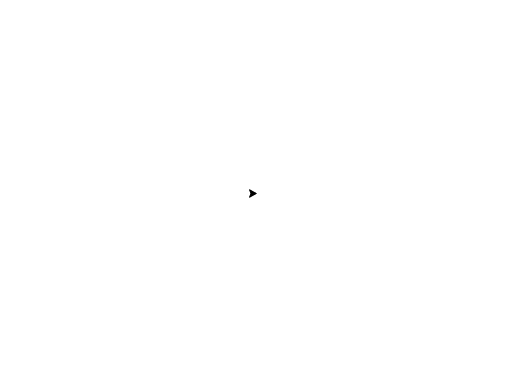
\includegraphics[width=10cm]{eps/turtle_doing_nothing.eps}}
\end{center}
We call \texttt{tom} an \textsl{instance} of a \turtle; \turtle is the class of
objects, \texttt{tom} is an example of it.

Here the turtle does something (\texttt{line.py}):
\begin{lstlisting}[numbers=left]
from turtle import *

tom=Turtle()

tom.forward(100)
\end{lstlisting}
The extra line, \lnn{5}, tells the turtle to move forward by 100
units, this is an important piece of Python syntax, to tell an object
to do something you use a dot followed by the command, here it tells
the \turtle called \texttt{tom} to perform the command
\texttt{forward}. Of course, the command has to make sense for
whatever type of object it is dotted onto, but here it does,
\texttt{forward} is one of the defined commands for a \turtle object;
we will see more of them as we go along, or google can provide a
list. Generally, commands that are associated with object, the
commands that you use with a dot, are called \textsl{methods}.
\begin{center}
\fbox{
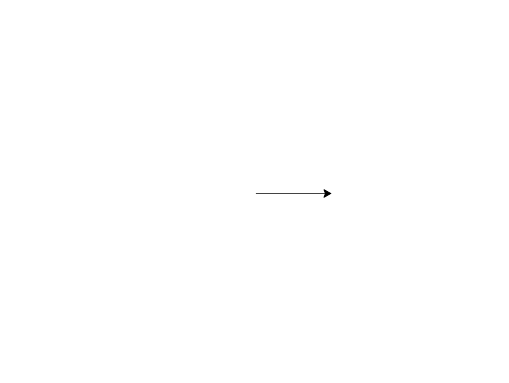
\includegraphics[width=10cm]{eps/line.eps}}
\end{center}

\turtle objects have another command \texttt{right(90)} which turns the turtle by $90^\circ$. QUESTION: Can you write a programme to draw this (\texttt{right\_angle.py}):
\begin{center}
\fbox{
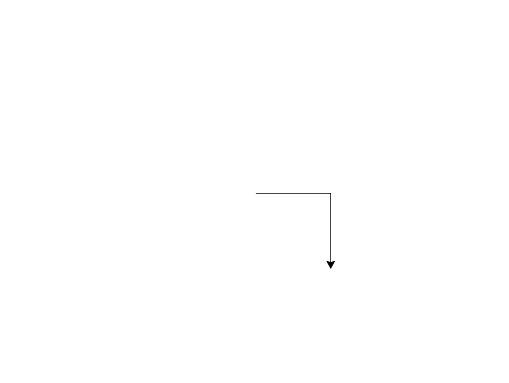
\includegraphics[width=10cm]{eps/right_angle.eps}}
\end{center}
QUESTION: How about a square?
\begin{center}
\fbox{
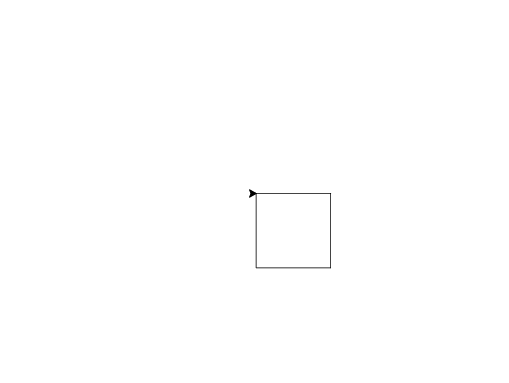
\includegraphics[width=10cm]{eps/square.eps}}
\end{center}

\subsection*{Flow control}

Perhaps you programme to draw a square looked like this
\begin{lstlisting}[numbers=left]
from turtle import *

tom=Turtle()

tom.forward(100)
tom.right(90)
tom.forward(100)
tom.right(90)
tom.forward(100)
tom.right(90)
tom.forward(100)
tom.right(90)
\end{lstlisting}
There are a few problems with this, most obviously it is boring
writing in the same two lines again and again; secondly, the programme
is inflexible and hard to read, we'll deal with the inflexible bit
later, but as for the hard to read, to know that it draws four lines
and has four corners you need to count the lines; it would be better
if the \lq{}fourness\rq{} was more apparent, as it is in this
programme (\texttt{square\_loop}):
\begin{lstlisting}[numbers=left]
from turtle import *

tom=Turtle()

for i in range(0,4):
   tom.forward(100)
   tom.right(90)

\end{lstlisting}
The business part of this program is \textbf{line 5};
\texttt{range(0,4)} is the list of numbers \texttt{[0,1,2,3]}, so
starting at zero and ending one before four; the full command says
that \texttt{i} takes each value in this list in turn and then does
all the stuff belonging to the command. Here the command is a
\texttt{for}, a command that says \lq{}do everything that belongs to
the me once for every value the variable, in this case i, is
instructed to take\rq{}. In Python stuff belonging to a command is
indented, so that means it does \lnn{6} and \lnn{7} once for each item
in the list: four times. The \lq{}stuff belong to a command\rq{} is
called the \textsl{block}, so in Python blocks are denoted with
indents.  

Of course, in this programme \texttt{i} isn't used for anything except
counting but it could be (\texttt{spiral1.py}):
\begin{lstlisting}[numbers=left]
from turtle import *

tom=Turtle()

for i in range(0,8):
   tom.forward(100+10*i)
   tom.right(90)

\end{lstlisting}
giving
\begin{center}
\fbox{
\includegraphics[width=10cm]{eps/spiral1.eps}}
\end{center}
\texttt{i} is \textsl{variable}, it stores some data, in this case a number
which changes each time the programme goes around the \texttt{for}
loop. One slightly confusing thing is \lq{}scoping\rq{}, which is
where the variable is defined; the \texttt{i} is only defined inside
the \texttt{for} loop, that is, it only exists while the programme is
executing \lnn{5} to \lnn{7}, but that's fine, that's where we use it.
QUESTION: Can you draw a triangular spiral like this:
\begin{center}
\fbox{
\includegraphics[width=10cm]{eps/spiral2.eps}}
\end{center}

The list in the \texttt{for} loop doesn't have to be a \texttt{range},
in this example (\texttt{square\_color.py})
\begin{lstlisting}[numbers=left]
from turtle import *

tom=Turtle()

colors=['red','green','blue','yellow']

for color in colors:
    tom.pencolor(color)
    tom.forward(100)
    tom.right(90)
\end{lstlisting}
\texttt{colors} defined in \lnn{5} is a list of colours and the
variable in the \texttt{for} command takes each of these values in
turn. \texttt{pencolor} is another \turtle method, it changes the pen
colour so we get
\begin{center}
\fbox{
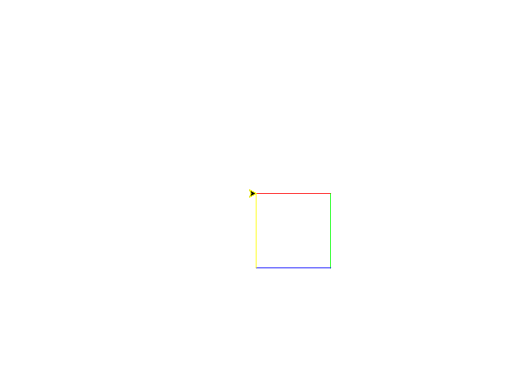
\includegraphics[width=10cm]{eps/square_color.eps}}
\end{center}

In the colour example we use a variable \texttt{colors} to store a
list; here is an example where we use a variable to store an integer
\texttt{n} which gives a number of sides.
\begin{lstlisting}[numbers=left]
from turtle import *

tom=Turtle()

n=8

for i in range(0,n):
    tom.forward(100)
    tom.right(360.0/n)

\end{lstlisting}
This is useful because we need the number of sides twice, once in
\lnn{7} where it gives the number of sides, and the second time in
\lnn{9} where it is used to calculate the turning angle. Obviously it
would be possible to write the number in those two places, but that
would be a very bad programming style because it would mean changing
it in those two places if you wanted to change the number of sides to
the polygon. It would be easy to get this wrong, maybe not for only
two places, but in a more complex programme there may be many places a
value needs to be changed, leading to errors. Furthermore, keeping
\texttt{n} seperate makes the programme easier to understand.

Here is a program for drawing a circle (\texttt{circle.py}); \turtle
has a function that draws a circle directly, but that seems like
cheating:
\begin{lstlisting}[numbers=left]
from turtle import *

tom=Turtle()

radius=100
step_size=2*3.141592*radius/360

for i in range(0,360):
    tom.forward(step_size)
    tom.right(1)
\end{lstlisting}
Notice the way the calculation of the step size from the radius is
done seperately in \lnn{5} and \lnn{6}; these calculations could've
put into the loop, directly in \lnn{9}, as in 
\begin{lstlisting}[numbers=left]
from turtle import *

tom=Turtle()

for i in range(0,360):
    tom.forward(2*3.141592*100/360)
    tom.right(1)
\end{lstlisting}
but this is more readible and easier to change.

Along with loops, the other important control statement is the
\texttt{if}. Consider a programme for drawing a star:
\begin{center}
\fbox{

\includegraphics[width=10cm]{eps/star.eps}}
\end{center}
The programme is
\begin{lstlisting}[numbers=left]
from turtle import *

tom=Turtle()

for i in range(0,10):
    tom.forward(100)
    if i%2==0:
        tom.right(144)
    else:
        tom.left(72)
\end{lstlisting}
The star has two different angles, every second line either has a
right turn of $144^\circ$ or a left turn of $72^\circ$. The
\texttt{if} on \lnn{7} decides which to do, basically \texttt{i\%2} is
the remainder you get if you divide \texttt{i} by two, so it is zero
if \texttt{i} is even and one if it is odd. Now \texttt{i\%2==0} tests
is \texttt{i\%2} is equal zero, the \texttt{==} is \lq{}is equal\rq{},
the \texttt{i\%2==0} returns true of false. In the if command, the
\texttt{if} is followed by a statement, if the statement is true, the
programme runs the code belonging to the if, if the statement is
false, it skips it. As ever, in Python, the indent is used to show
belonging. An if command needn't have an else, but this one does, the
code belonging to \texttt{else} runs if the statement in the
\texttt{if} is false. All this means \texttt{tom} does one turn for
even \texttt{i} and another for odd. QUESTION: can you modify the code
to give a six-pointed star, the two angles you need are $120^\circ$
and $60^\circ$
\begin{center}
\fbox{
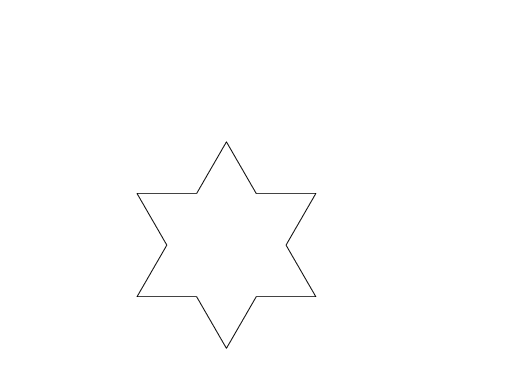
\includegraphics[width=10cm]{eps/six_star.eps}}
\end{center}

\subsection*{Functions}

Now imagine you wanted to draw this:
\begin{center}
\fbox{
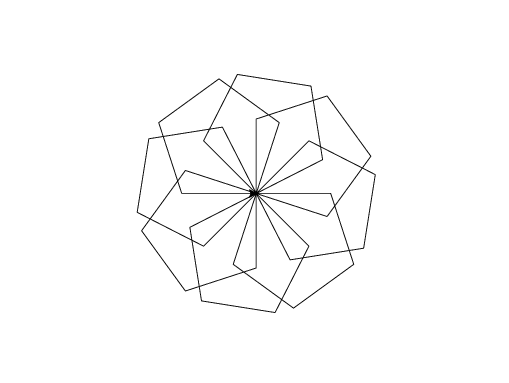
\includegraphics[width=10cm]{eps/many_polygons.eps}}
\end{center}
This is made of eight pentagons with an eighth of a full turn between
each one; this can be made using the programme:
\begin{lstlisting}[numbers=left]
from turtle import *

tom=Turtle()

repeats=8
polygon_sides=5

for i in range(0,repeats):
   for j in range(0,polygon_sides):
       tom.forward(100)
       tom.right(360.0/polygon_sides)
   tom.right(360/repeats)
\end{lstlisting}
So this programme has two \texttt{for} loops, the \texttt{j} loop from
\lnn{8} to \lnn{10} draws the pentagons, the \texttt{i} loop repeats
that eight times and rotates between pentagon. Notice the two loops
need different variables, \texttt{i} and \texttt{j}, and you can tell
what belongs to which loop by the indent, \lnn{9} and \lnn{10} belong
to the \texttt{j} loop so these command are run $40=8\times 5$ times
whereas \lnn{9} and \lnn{11} are only run eight times.

This programme works, but it fails our readibility and adaptability
test; to work out what it does you need to figure your way through the
double loop and if you wanted to draw another pentagon later you would
have to cut and paste the lines you already had. A much better
programme would use a function (\texttt{many\_polygons.py}):
\begin{lstlisting}[numbers=left]
from turtle import *

def polygon(n):

    for i in range(0,n):
        tom.forward(100)
        tom.right(360.0/n)

tom=Turtle()

repeats=8
polygon_sides=5

for i in range(0,repeats):
    polygon(polygon_sides)
    tom.right(360.0/repeats)
\end{lstlisting}
Now in \lnn{3} to \lnn{7} we have defined a \texttt{function}, the
command \texttt{def} announces in \lnn{3} that a function definition
is on the way, all the indented lines are the definition. The function
is named \texttt{polygon}; the brackets after the function name are to
give the arguements, values that are sent to the function, in this
case the function has one arguement which will give the number of
sides of the polygon. Now we have a new command, \texttt{polygon(n)},
whenever the command is given, the programme goes up to the function
and runs the code belonging to the function, this happens in \lnn{17}.

QUESTION: can you guess how this was drawn:
\begin{center}
\fbox{
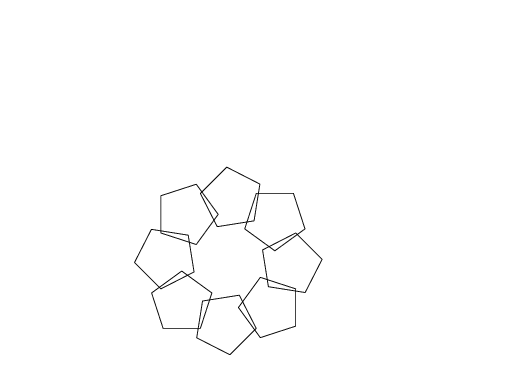
\includegraphics[width=10cm]{eps/many_polygons_extra.eps}}
\end{center}
The \turtle commands \texttt{penup()} and \texttt{pendown()} lift and
drop the turtle's pen, when the pen is up the turtle moves without
leaving a line; \texttt{hideturtle()} hides the turtle (\texttt{many\_polygons\_extra.py})
A more complicated example (\texttt{vanishing\_square.py})
\begin{center}
\fbox{
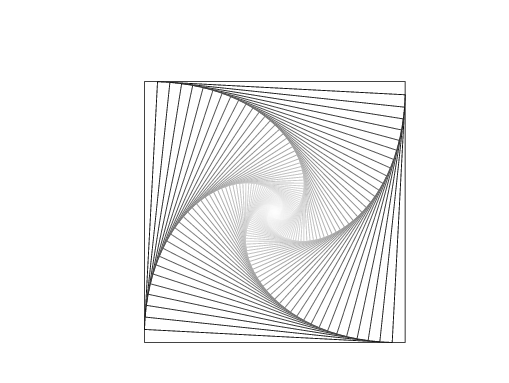
\includegraphics[width=10cm]{eps/vanishing_square.eps}}
\end{center}

\subsection*{Classes}

Throughout this worksheet we've been using the \turtle object but
haven't considered what we mean by an object; in fact it is a
\textsl{class}. In \textsl{Object Oriented Programming Languages} it
is possible to define objects, an object is a some data and some
methods that can act on that data. There isn't room here to go into
this in detail but here is an example:
\begin{lstlisting}[numbers=left]
from turtle import *

class Colors:
    
    def __init__(self,color_v):
        self.color_v=color_v
        self.current=0

    def change_colour(self,jacob):
        self.current+=1
        if self.current==len(self.color_v):
            self.current=0
        jacob.color(self.color_v[self.current])

def curve(arc_length, curvature,steps,jacob):
    small_arc=arc_length/steps
    small_curve=curvature/steps
    for i in range(steps):
        jacob.forward(small_arc)
        jacob.right(small_curve)


jacob=Turtle()
colors=Colors(['green','red','blue','yellow','orange','black'])

for i in range(0,12):
    curve(200,40,30,jacob)
    curve(40,120,10,jacob)
    colors.change_colour(jacob)
\end{lstlisting}
which draws this
\begin{center}
\fbox{
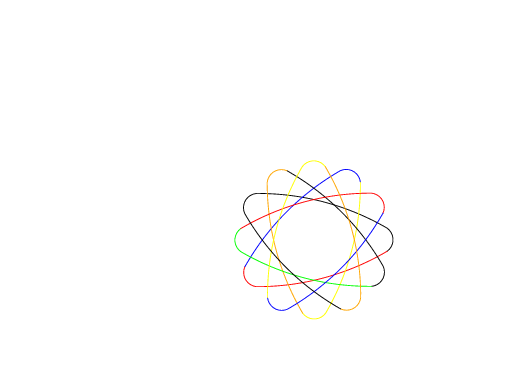
\includegraphics[width=10cm]{eps/spirograph.eps}}
\end{center}
The class is defined at the top, starting at \lnn{3}. This object is
for choosing the next colour in a drawing, it remembers the list of
colours and the current colour. When a Class is being defined, the
data is called \texttt{self}, so \texttt{self.color} and
\texttt{self.current} are variables belonging to the Class. Now an
instance of a class has a name, here we make an example of
\texttt{Colors} at \lnn{27}, the instance is called \texttt{colors}
with a small c, it could've been named anything. Now to get the value
of \texttt{current} for this instance, we would write
\texttt{colors.current}; the \texttt{self} stands in for the name of
the object in the general definition. Either way, without going into
details, the \texttt{\_\_init\_\_} function is a method explaining how
to make an instance of \texttt{Colours} and \texttt{change\_colour} is
a method for changing the colour of the turtle so that the turtle gets
the next colour on the list, if the index gets too big it gets reset
so the colours go around and around.

\end{document}

